% \documentclass{book}

\documentclass[12pt]{article}
\usepackage[pdfborder={0 0 0.5 [3 2]}]{hyperref}%
\usepackage[left=1in,right=1in,top=1in,bottom=1in]{geometry}%
\usepackage[shortalphabetic]{amsrefs}%
\usepackage{amsmath}
\usepackage{enumerate}
\usepackage{enumitem}
\usepackage{amssymb}                
\usepackage{amsmath}                
\usepackage{amsfonts}
\usepackage{amsthm}
\usepackage{bbm}
\usepackage[table,xcdraw]{xcolor}
\usepackage{tikz}
\usepackage{float}
\usepackage{svg}
\usepackage{mathtools}
\usepackage{cool}
\usepackage{url}
\usepackage{graphicx,epsfig}
\usepackage{makecell}
\usepackage{array}

\def\noi{\noindent}
\def\T{{\mathbb T}}
\def\R{{\mathbb R}}
\def\N{{\mathbb N}}
\def\C{{\mathbb C}}
\def\Z{{\mathbb Z}}
\def\P{{\mathbb P}}
\def\E{{\mathbb E}}
\def\Q{\mathbb{Q}}
\def\ind{{\mathbb I}}

\graphicspath{ {images/} }
\renewcommand{\arraystretch}{3}

\begin{document}

\begin{enumerate}
\item (10 points) 12 Brown undergraduate students -- 6 sophomores and 6 juniors -- enter the housing lottery. Suppose the students will live together in triples (groups of three) and are grouped into these triples uniformly at random.
\begin{enumerate}
\item How many possible arrangements are there of the 12 students into these triples?\\

You are dividing 12 students into 4 groups of 3. Using the multinomial coefficient, there are:
\[
\binom{12}{3\:3\:3\:3} = \frac{12!}{3!\:3!\:3!\:3!}
\]
ways to do this. But the multinomial divides the 12 students into 4 \emph{distinct} groups of 3, i.e. order matters. Thus since there are 4 groups, we divide by $4!$, the number of ways of permuting 4 groups (i.e. $4p4$) to get:
\[
\frac{12!}{4!\:3!\:3!\:3!\:3!}
\]
arrangements.
\item What is the probability that no triple contains both sophomores and juniors? \\
For this to happen, two triples must contain only sophomores, and two triple must contain only juniors. The number of ways to arrange 6 sophomores into 2 triples, where order does not matter is:
\[
\frac{6!}{2!\:3!\:3!}
\]
where we have used the multinomial and divided by $2!$ since order does not matter, i.e. the triples are not distinct. The number of ways to arrange the 6 juniors into 2 triples is exactly the same. Thus the number of ways of arranging the 12 students into 4 triples where all triples contain students from only one class is:
\[
\frac{6!}{2!\:3!\:3!}\frac{6!}{2!\:3!\:3!}
\]
\end{enumerate}
To get the probability of this occurring, we divide by the result in part (a), which is the size of the sample space:
\[
\dfrac{\frac{6!}{2!\:3!\:3!}\frac{6!}{2!\:3!\:3!}}{\frac{12!}{4!\:3!\:3!\:3!\:3!}}
\]

\pagebreak

\item (10 points) Your friend has a bag of 3 six-sided dice. One of the dice is loaded so that the probability that it rolls a 6 is 1/2 (the rest of the numbers are rolled uniformly at random). The remaining two dice are standard, fair dice. You draw one of the dice from the bag uniformly at random and roll it.
\begin{enumerate}
\item If your roll is a 6, what is the probability that you rolled the unfair die?\\

There are many ways of doing this, but we will use Bayes' rule (you can also draw a tree). Let $S$ be the event that a 6 is rolled, and $U$ the event that you chose the unfair die from the bag. We are interested in $P(U|S)$. By Bayes' rule and the Law of Total Probability:
\begin{align*}
\P(U|S) &= \frac{ \P(S|U)\P(U) }{ \P(S) } \\
&= \frac{ \P(S|U)\P(U) }{ \P(S|U)\P(U) + \P(S|U^c)\P(U^c) }\\
&= \frac{ (1/2)(1/3) }{ (1/2)(1/3) + (1/6)(2/3) } \\
&= \frac{ 1/6 }{ 1/6 + 1/9 } \\
&= \frac{ 1/6 }{ 5/18 } \\
&= \frac{3}{5}
\end{align*}
\item If you then roll the same die again, what is the probability that it will roll a 6?\\

From (a), the probability that you are holding the unfair die is 3/5. Let $A$ be the event that you are holding the unfair die (technically this is conditional on seeing a 6 for the first roll, but we will not include that in our notation for simplicity). Let $T$ be the event that we roll a 6 on the second roll. Using a tree or the law of total probability:
\begin{align*}
\P(T) &= \P(T|A)\P(A) + \P(T|A^c)\P(A^c) \\
&= (1/2)(3/5) + (1/6)(2/5) \\
&= 11/30
\end{align*}

\end{enumerate} 

\pagebreak

\item (10 points) The ICERM building downtown has 11 floors (numbered 1 - 11). Suppose $m$ people enter the elevator on floor 1 and each one independently and uniformly at random chooses a floor between 2 and 11 (inclusive). What is the expected number of stops of the elevator?\\

Let $X$ be the number of floors the elevators stops at. Define indicator random variables $X_2, \dots, X_{11}$ by:
\[
X_i = \begin{cases}
1 & \text{elevator stops at floor $i$}\\
0 & \text{elevator does not stop at floor $i$}
\end{cases}
\]
Then $X = X_2 + \cdots + X_{11}$ and by linearity of expectation,
\[
\E(X) = \E(X_2) + \cdots + \E(X_{11})
\]
Computing one of the individual expected values:
\begin{align*}
\E(X_i) &= 0 \cdot \P(X_i = 1) + 1 \cdot \P(X_i = 1) \\
&= \P(X_i = 1)
&= 1 - \P(X_i = 0)
\end{align*}
If $X_i = 0$, the elevator does not stop on floor $i$. This means that all of the $m$ people select one of the other 9 floors (out of 10 total floors). Since the elevator floors are selected uniformly at random and the selections of each of the $m$ people are independent, we have:
\[
\P(X_i = 0) = \left( \frac{9}{10} \right)^m
\]
Putting this together, we have:
\begin{align*}
\E(X) = \underbrace{ \left(1 - \left( \frac{9}{10} \right)^m \right) + \cdots + \left(1 - \left( \frac{9}{10} \right)^m \right) }_{\text{10 terms in sum}}
&= 10 \left(1 - \left( \frac{9}{10} \right)^m \right)
\end{align*}
Alternately, you could use the binomial distribution. Each floor is a Bernoulli trial, and stopping on a floor is a ``success''. The probability of \emph{not} stopping on a given floor is $(9/10)^m$, as we found above, so the probability of stopping on a given floor is $p = 1 - (9/10)^m$. Then $X \sim\text{Binomial}(10, 1 - (9/10)^m)$. Since the expected value of a binomial random variable is $np$, we have $\E(X) = 10( 1 - (9/10)^m) $.

\pagebreak

\item (10 points) You have two bags of marbles. Bag 1 contains 1 white marble and 5 red marbles. Bag 2 contains 5 white marbles and 1 red marble. You remove a marble uniformly at random from bag 1 and put it into bag 2. Then you remove a marble uniformly at random from bag 2 and put it back into bag 1. You do not look at the marble either time. At the end of this, what is the probability that the two bags have their original configurations (i.e. Bag 1 contains 1 white and 5 red marbles, Bag 2 contains 5 white and 1 red marbles)?\\

This is easiest to do with a tree diagram. Let $W_1$ and $R_1$ be the events that a white or a red marble is chosen (from bag 1) on the first draw. Let $W_2$ and $R_2$ be the events that a white or a red marble is chosen (from bag 2) on the second draw. Then we have the following tree diagram.

\begin{figure}[H]
\centering
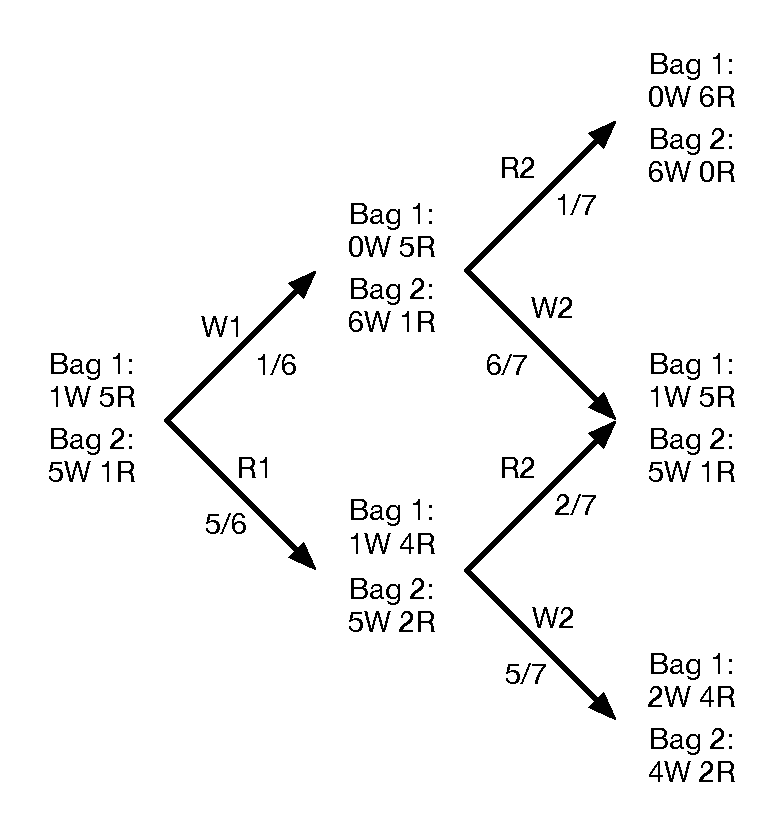
\includegraphics[width=8cm]{exam1tree}
\end{figure}

Multiplying the appropriate probabilities and adding them up we get:
\begin{align*}
\P(\text{same configuration at end}) = (1/6)(6/7) + (5/6)(2/7) = 8/21
\end{align*}

\pagebreak

\item (10 points) The Red Rose Tea company sells boxes of tea. Each box comes with a collectible figurine! There are $n$ total figurines, which are distributed uniformly at random in the boxes. You have already collected $m$ of them.
\begin{enumerate}
\item Suppose you buy $b$ boxes of tea. What is the probability that at least one of them contains a new figurine?\\

Since you have already collected $m$ figurines, there are $n-m$ figurines left to collect. Thus each purchase of a box is a Bernoulli trial, with probability of success $p = (n - m)/n = 1 - m/n $. Let $X$ be the number of boxes (out of a total of $b$ boxes) which contains a new figurine. Then $X \sim\text(Binomial(b, 1 - m/n)$. We want $\P(X \geq 1)$, which is given by:
\begin{align*}
\P(X \geq 1) &= 1 - \P(X = 0) \\
&= 1 - \binom{b}{0} (1 - m/n)^0 [1 - (1 - m/n)]^{b - 0}\\
&= 1 - (m/n)^b
\end{align*}
A pure combinatorial argument works as well.

\item What is the expected number of boxes you need to buy until you get a new figurine?\\

Let $Y$ be the number of boxes until you get a new figurine. Then with the same setup above, $Y \sim\text{Geometric}(1 - m/n)$. Thus:
\begin{align*}
\E(Y) &= \frac{1}{p} = \frac{1}{1 - m/n} = \frac{n}{n-m}
\end{align*}
\item What is the expected number of boxes you need to buy until you have collected all the figurines? \\

Note that you have $n-m$ figurines left to collect. Let $Y_1$ be the number of boxes until you get the first new figurine. After we get the first new figurine, let $Y_2$ be the number of additional boxes it takes to get the second new figurine. After we get the first two new figurines let $Y_3$ be the number of additional boxes it takes to get the third new figurine. Repeat this until we get $Y_{n-m}$, the number of additional boxes it takes to get the $(n-m)$th new figurine, which is the final one in the collection. Then:
\begin{itemize}
\item $Y_1 \sim\text{Geometric}((n-m)/n)$
\item $Y_2 \sim\text{Geometric}((n - (m + 1)/n) = \text{Geometric}((n - m - 1)/n)$\\
\item $Y_3 \sim\text{Geometric}((n - (m + 2)/n) = \text{Geometric}((n - m - 2)/n)$\\
\vdots\\
\item $Y_{n-m} \sim\text{Geometric}(1/n)$
\end{itemize}
Let $Y$ be the number of boxes it takes to collect all the figurines. Then
\[
Y = Y_1 + Y_2 + Y_3 + \cdots + Y_{n-m}
\]
By linearity of expectation
\begin{align*}
\E(Y) &= \E(Y_1) + \E(Y_2) + \E(Y_3) + \cdots + \E(Y_{n-m}) \\
&= \frac{1}{(n-m)/n)} + \frac{1}{(n - m - 1)/n} + \frac{1}{(n - m - 2)/n} + \cdots + \frac{1}{1/n} \\
&=  \frac{n}{n-m} + \frac{n}{n - m - 1)} + \frac{n}{n - m - 2} + \cdots + n \\
&= n\left(1 + \frac{1}{2} + \frac{1}{3} + \cdots + \frac{1}{n-m-1} + \frac{1}{n-m}  \right)
\end{align*}

\end{enumerate}

\end{enumerate}




\end{document}

